\documentclass[12pt,a4paper,titlepage]{article}
\usepackage[a4paper]{geometry}
\usepackage[utf8]{inputenc}
\usepackage[english]{babel}
\usepackage{lipsum}
\usepackage{graphicx}
\graphicspath{ {images/} }
\usepackage[export]{adjustbox}

\usepackage{amsmath, amssymb, amsfonts, amsthm, fouriernc, mathtools}
% mathtools for: Aboxed (put box on last equation in align envirenment)
\usepackage{microtype} %improves the spacing between words and letters

\usepackage{epsfig}
\usepackage{epstopdf}


%%%%%%%%%%%%%%%%%%%%%%%%%%%%%%%%%%%%%%%%%%%%%%%%%%
%% COLOR DEFINITIONS
%%%%%%%%%%%%%%%%%%%%%%%%%%%%%%%%%%%%%%%%%%%%%%%%%%
\usepackage[svgnames]{xcolor} % Enabling mixing colors and color's call by 'svgnames'
%%%%%%%%%%%%%%%%%%%%%%%%%%%%%%%%%%%%%%%%%%%%%%%%%%
\definecolor{MyColor1}{rgb}{0.2,0.4,0.6} %mix personal color
\newcommand{\textb}{\color{Black} \usefont{OT1}{lmss}{m}{n}}
\newcommand{\blue}{\color{MyColor1} \usefont{OT1}{lmss}{m}{n}}
\newcommand{\blueb}{\color{MyColor1} \usefont{OT1}{lmss}{b}{n}}
\newcommand{\red}{\color{LightCoral} \usefont{OT1}{lmss}{m}{n}}
\newcommand{\green}{\color{Turquoise} \usefont{OT1}{lmss}{m}{n}}
%%%%%%%%%%%%%%%%%%%%%%%%%%%%%%%%%%%%%%%%%%%%%%%%%%




%%%%%%%%%%%%%%%%%%%%%%%%%%%%%%%%%%%%%%%%%%%%%%%%%%
%% FONTS AND COLORS
%%%%%%%%%%%%%%%%%%%%%%%%%%%%%%%%%%%%%%%%%%%%%%%%%%
%    SECTIONS
%%%%%%%%%%%%%%%%%%%%%%%%%%%%%%%%%%%%%%%%%%%%%%%%%%
\usepackage{titlesec}
\usepackage{sectsty}
%%%%%%%%%%%%%%%%%%%%%%%%
%set section/subsections HEADINGS font and color
\sectionfont{\color{MyColor1}}  % sets colour of sections
\subsectionfont{\color{MyColor1}}  % sets colour of sections

%set section enumerator to arabic number (see footnotes markings alternatives)
\renewcommand\thesection{\arabic{section}.} %define sections numbering
\renewcommand\thesubsection{\thesection\arabic{subsection}} %subsec.num.

%define new section style
\newcommand{\mysection}{
\titleformat{\section} [runin] {\usefont{OT1}{lmss}{b}{n}\color{MyColor1}} 
{\thesection} {3pt} {} } 

%%%%%%%%%%%%%%%%%%%%%%%%%%%%%%%%%%%%%%%%%%%%%%%%%%
%		CAPTIONS
%%%%%%%%%%%%%%%%%%%%%%%%%%%%%%%%%%%%%%%%%%%%%%%%%%
\usepackage{caption}
\usepackage{subcaption}
%%%%%%%%%%%%%%%%%%%%%%%%
\captionsetup[figure]{labelfont={color=Turquoise}}

%%%%%%%%%%%%%%%%%%%%%%%%%%%%%%%%%%%%%%%%%%%%%%%%%%
%		!!!EQUATION (ARRAY) --> USING ALIGN INSTEAD
%%%%%%%%%%%%%%%%%%%%%%%%%%%%%%%%%%%%%%%%%%%%%%%%%%
%using amsmath package to redefine eq. numeration (1.1, 1.2, ...) 
%%%%%%%%%%%%%%%%%%%%%%%%
\renewcommand{\theequation}{\thesection\arabic{equation}}

%set box background to grey in align environment 
\usepackage{etoolbox}% http://ctan.org/pkg/etoolbox
\makeatletter
\patchcmd{\@Aboxed}{\boxed{#1#2}}{\colorbox{black!15}{$#1#2$}}{}{}%
\patchcmd{\@boxed}{\boxed{#1#2}}{\colorbox{black!15}{$#1#2$}}{}{}%
\makeatother
%%%%%%%%%%%%%%%%%%%%%%%%%%%%%%%%%%%%%%%%%%%%%%%%%%




%%%%%%%%%%%%%%%%%%%%%%%%%%%%%%%%%%%%%%%%%%%%%%%%%%
%% DESIGN CIRCUITS
%%%%%%%%%%%%%%%%%%%%%%%%%%%%%%%%%%%%%%%%%%%%%%%%%%
\usepackage[siunitx, american, smartlabels, cute inductors, europeanvoltages]{circuitikz}
%%%%%%%%%%%%%%%%%%%%%%%%%%%%%%%%%%%%%%%%%%%%%%%%%%



\makeatletter
\let\reftagform@=\tagform@
\def\tagform@#1{\maketag@@@{(\ignorespaces\textcolor{red}{#1}\unskip\@@italiccorr)}}
\renewcommand{\eqref}[1]{\textup{\reftagform@{\ref{#1}}}}
\makeatother
\usepackage{hyperref}
\hypersetup{colorlinks=true}

%%%%%%%%%%%%%%%%%%%%%%%%%%%%%%%%%%%%%%%%%%%%%%%%%%
%% PREPARE TITLE
%%%%%%%%%%%%%%%%%%%%%%%%%%%%%%%%%%%%%%%%%%%%%%%%%%
\title{\blue Data Mining \\
\blueb Assignment Solution $2$}
\author{Vivek Patani}
\date{\today}
%%%%%%%%%%%%%%%%%%%%%%%%%%%%%%%%%%%%%%%%%%%%%%%%%%



\begin{document}
\maketitle
\textit{Please read readme.md for code execution directions, I have tried to maintain a generic structure for each question in coding terms.}
\section{Question 1 Solution}{Download data set Iris and answer the following questions:
}
{%
\subsection{Section 1}{ Calculate the average value and standard deviation for each of the four features.\\~\\
\centerline{Average for Petal Width: 1.2}~\\
\centerline{Variance for Petal Width: 0.58}~\\
\centerline{Standard Deviation for Petal Width: 0.762}~\\~\\
\centerline{Average for Petal Length: 3.76}~\\
\centerline{Variance for Petal Length: 3.09}~\\
\centerline{Standard Deviation for Petal Length: 1.758}~\\~\\
\centerline{Average for Sepal Length: 5.84}~\\
\centerline{Variance for Sepal Length: 0.68}~\\
\centerline{Standard Deviation for Sepal Length: 0.82}~\\~\\
\centerline{Average for Sepal Width: 3.05}~\\
\centerline{Variance for Sepal Width: 0.19}\\
\centerline{Standard Deviation for Sepal Width: 0.436}~\\~\\

\centerline{\textbf{Code Located in q1/q1.py}}
%%% END UBSECTION 1 %%%%%%%%%%%%%%%%%%%%%%%%%%%%%%%%%%%%%%
\subsection{Section 2}{
~\\
\centerline{Repeat the previous step but separately for each type of flower.}\\~\\
\centerline{Average for Sepal Width \& Iris Setosa: 3.42}\\
\centerline{Variance for Sepal Width \& Iris Setosa: 0.14}~\\
\centerline{Standard Deviation for Sepal Width \& Iris Setosa: 0.37416573867739417}~\\~\\
\centerline{Average for Sepal Length \& Iris Setosa: 5.01}~\\
\centerline{Variance for Sepal Length \& Iris Setosa: 0.12}~\\
\centerline{Standard Deviation for Sepal Length \& Iris Setosa: 0.34641016151377546}~\\~\\
\centerline{Average for Petal Width \& Iris Setosa: 0.24}~\\
\centerline{Variance for Petal Width \& Iris Setosa: 0.01}~\\
\centerline{Standard Deviation for Petal Width \& Iris Setosa: 0.1}~\\~\\
\centerline{Average for Petal Length \& Iris Setosa: 1.46}~\\
\centerline{Variance for Petal Length \& Iris Setosa: 0.03}~\\
\centerline{Standard Deviation for Petal Length \& Iris Setosa: 0.17320508075688773}~\\~\\
\centerline{Average for Sepal Width \& Iris Versicolor: 2.77}~\\
\centerline{Variance for Sepal Width \& Iris Versicolor: 0.1}~\\
\centerline{Standard Deviation for Sepal Width \& Iris Versicolor: 0.31622776601683794}~\\~\\
\centerline{Average for Sepal Length \& Iris Versicolor: 5.94}~\\
\centerline{Variance for Sepal Length \& Iris Versicolor: 0.26}~\\
\centerline{Standard Deviation for Sepal Length \& Iris Versicolor: 0.5099019513592785}~\\~\\
\centerline{Average for Petal Width \& Iris Versicolor: 1.33}~\\
\centerline{Variance for Petal Width \& Iris Versicolor: 0.04}~\\
\centerline{Standard Deviation for Petal Width \& Iris Versicolor: 0.2}~\\~\\
\centerline{Average for Petal Length \& Iris Versicolor: 4.26}~\\
\centerline{Variance for Petal Length \& Iris Versicolor: 0.22}~\\
\centerline{Standard Deviation for Petal Length \& Iris Versicolor: 0.469041575982343}~\\~\\
\centerline{Average for Sepal Width \& Iris Virginica: 2.97}~\\
\centerline{Variance for Sepal Width \& Iris Virginica: 0.1}~\\
\centerline{Standard Deviation for Sepal Width \& Iris Virginica: 0.31622776601683794}~\\~\\
\centerline{Average for Sepal Length \& Iris Virginica: 6.59}~\\
\centerline{Variance for Sepal Length \& Iris Virginica: 0.4}~\\
\centerline{Standard Deviation for Sepal Length \& Iris Virginica: 0.6324555320336759}~\\~\\
\centerline{Average for Petal Width \& Iris Virginica: 2.03}~\\
\centerline{Variance for Petal Width \& Iris Virginica: 0.07}~\\
\centerline{Standard Deviation for Petal Width \& Iris Virginica: 0.2645751311064591}~\\~\\
\centerline{Average for Petal Length \& Iris Virginica: 5.55}~\\
\centerline{Variance for Petal Length \& Iris Virginica: 0.3}~\\
\centerline{Standard Deviation for Petal Length \& Iris Virginica: 0.5477225575051661}~\\~\\
}\label{sub:sub2}%
%%% END SUBSECTION 2 %%%%%%%%%%%%%%%%%%%%%%%%%%%%%%%%%%%%%
\subsection{Section 3}{
Draw four box plots, one for each feature, such that each figure shows three boxes, one for each type of flower. Properly label your figures and axes in all box plots. Make sure that the box plots look professional and appear in high resolution. Experiment with thickness of lines, font styles/sizes, etc. and describe what you tried and what looked the most professional.\\
\centering
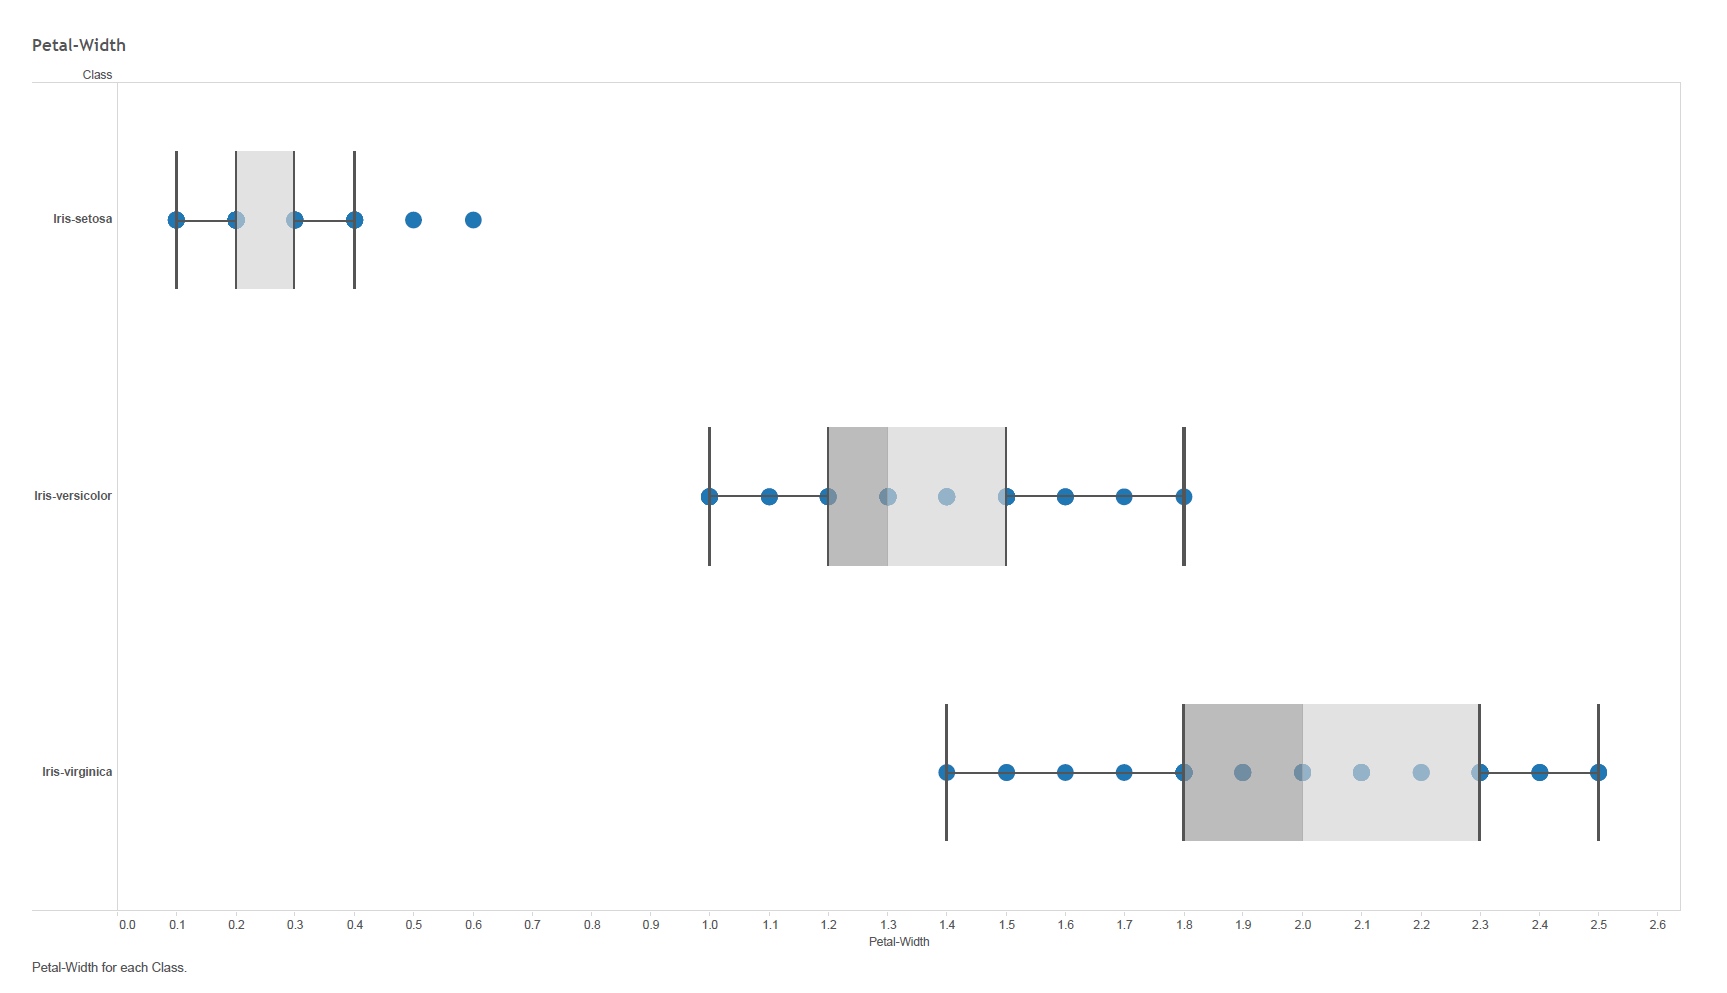
\includegraphics[max size={\textwidth}{\textheight}]{petal-width}\\
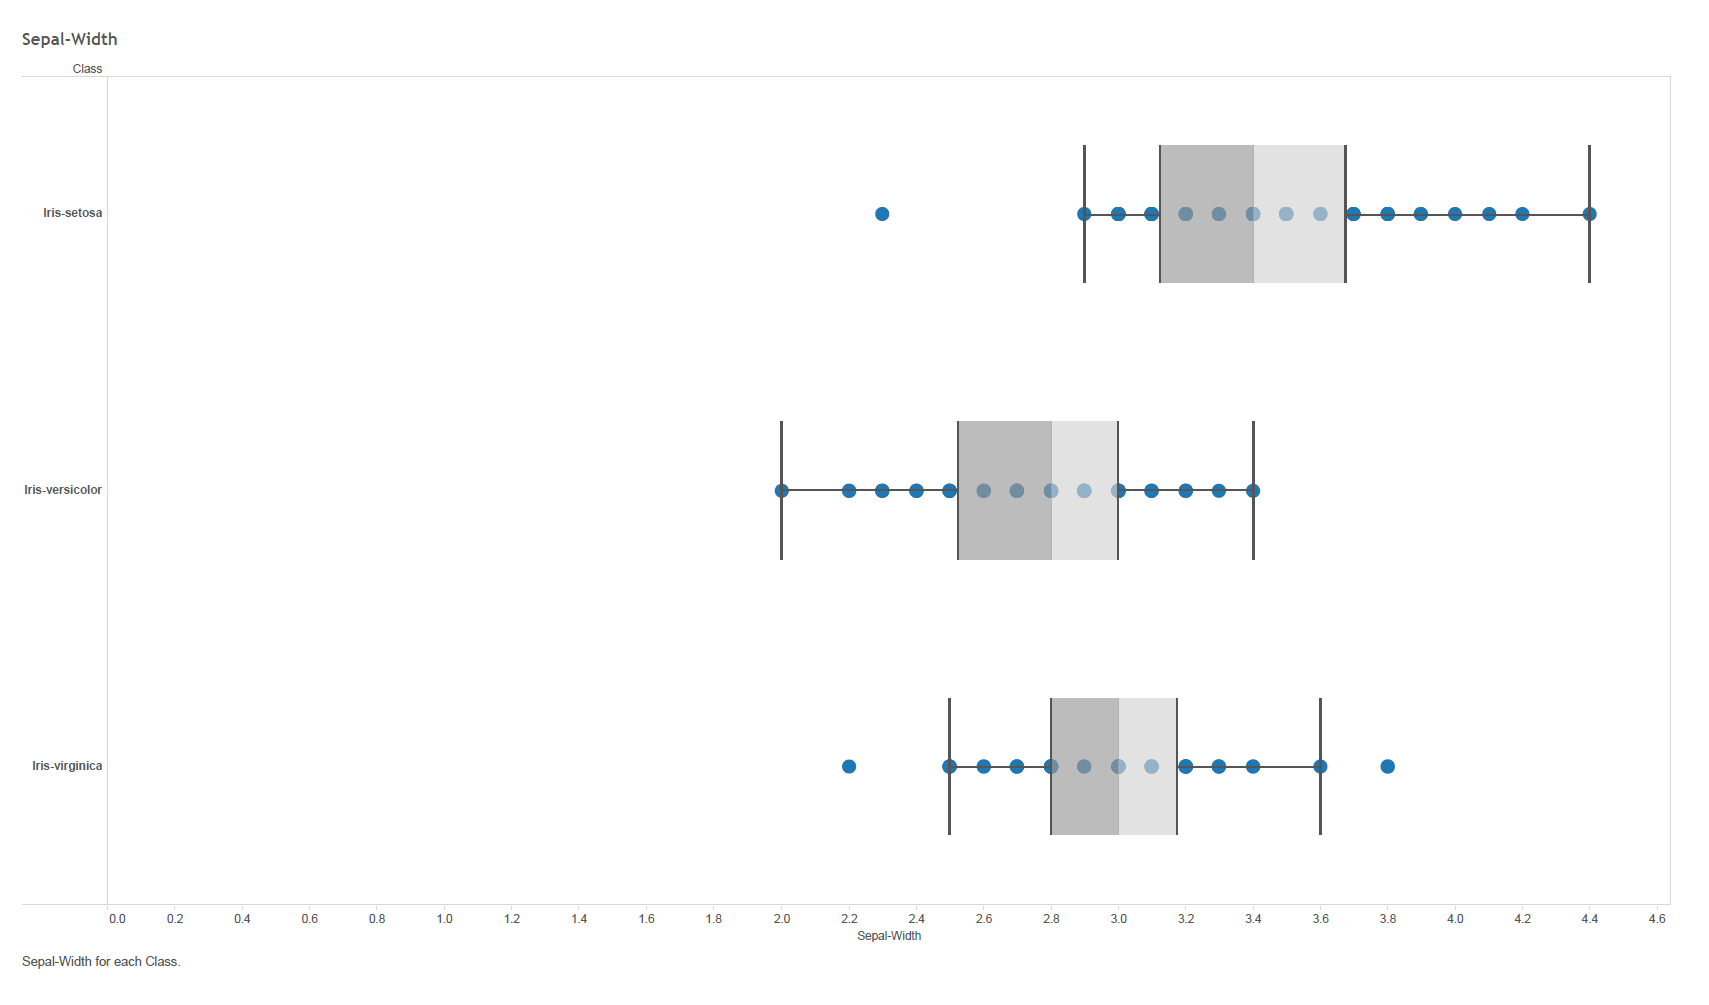
\includegraphics[max size={\textwidth}{\textheight}]{sepal-width}\\
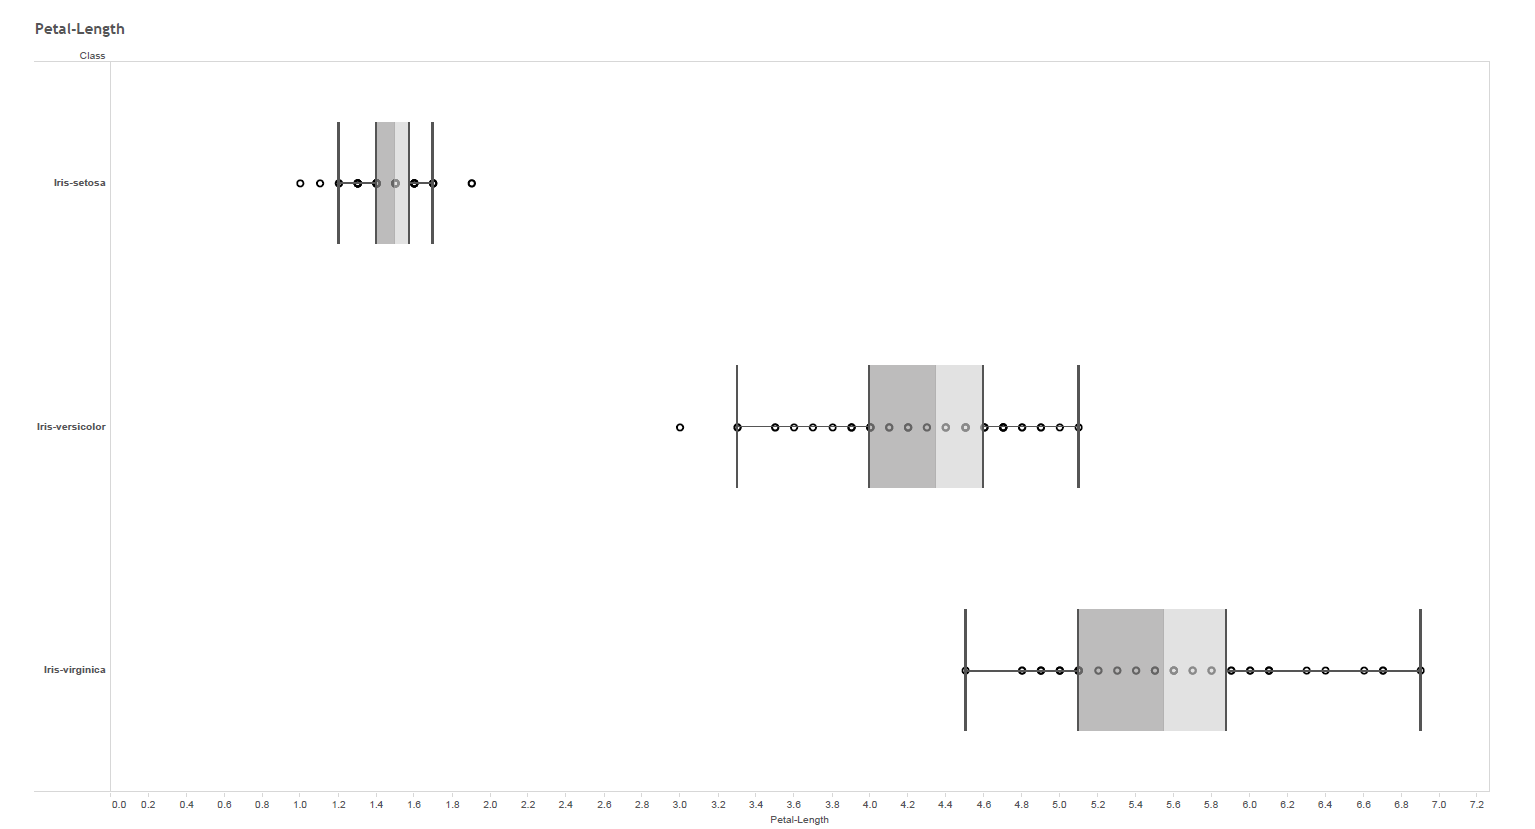
\includegraphics[max size={\textwidth}{\textheight}]{petal-length}\\
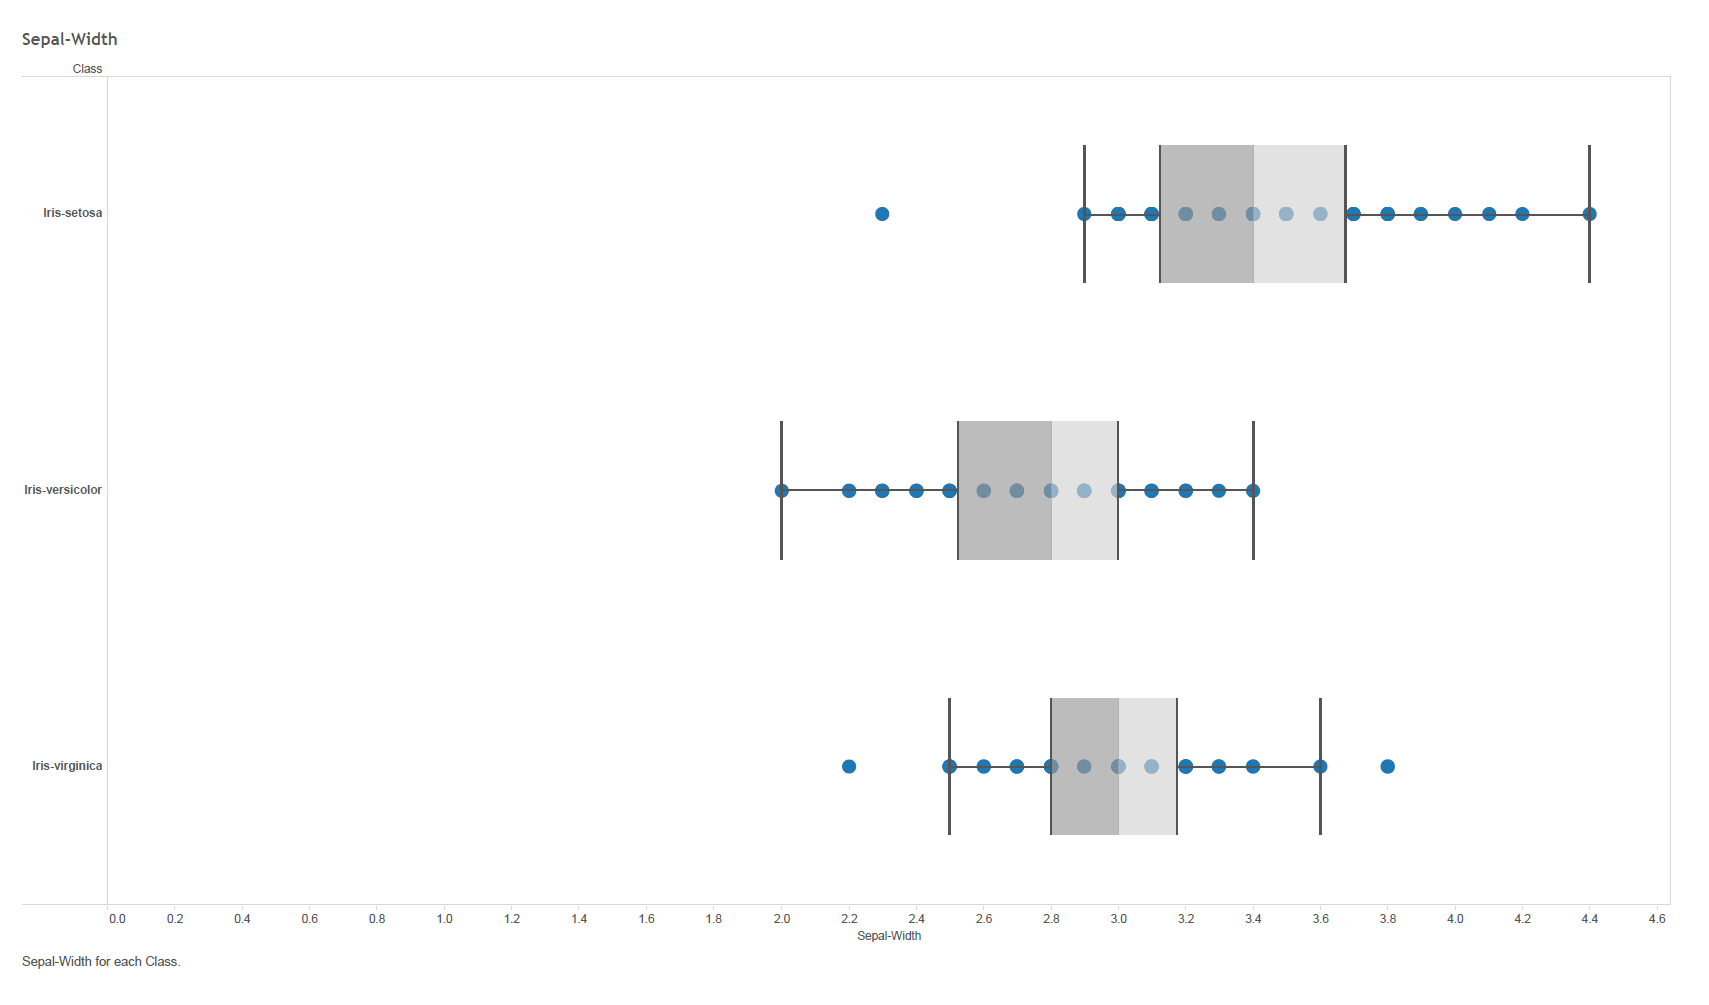
\includegraphics[max size={\textwidth}{\textheight}]{sepal-width}\\
}\label{sub:sub3}
%%% END SUBSECTION 3 %%%%%%%%%%%%%%%%%%%%%%%%%%%%%%%%%%%%%
}
%%% END SECTION 1 %%%%%%%%%%%%%%%%%%%%%%%%%%%%%%%%%%%%%%%



\section{Question 2 Solution}{
Download data set Wine and answer the following questions
\subsection{Section 1}{
Provide pairwise scatter plots for four most correlated and four least correlated pairs of features, using Pearson's correlation coefficient. Label all axes in all your plots and select fonts of appropriate style and size. Experiment with different ways to plot these scatter plots and choose the one most visually appealing and most professionally looking.

}

%%% END SUBSECTION 1 %%%%%%%%%%%%%%%%%%%%%%%%%%%%%%%%%%%%%%
\subsection{Section 2}{
Use Euclidean distance to find the closest example to every example available in the data set (exclude the class variable). Calculate the percentage of points whose closest neighbours have the same class label (for data set as a whole and also for each class).
}
%%% END SUBSECTION 2 %%%%%%%%%%%%%%%%%%%%%%%%%%%%%%%%%%%%%%

\subsection{Section 3}{
Repeat the previous step but after the data set is normalized using first 0-1 normalization and then z-score normalization. Investigate the reasons for discrepancy and provide evidence to support every one of your claims. Provide the code you used for normalizing and visualizing the data.
}
%%% END SUBSECTION 3 %%%%%%%%%%%%%%%%%%%%%%%%%%%%%%%%%%%%%%
%%% END SECTION 2 %%%%%%%%%%%%%%%%%%%%%%%%%%%%%%%%%%%%%%%%



\section{Question 3 Solution}{
Data exploration is often the first step in many data analysis tasks. Visualizing relationships between features as well as between features and the target variable(s), for example, can be exploited to design a good model or to understand why a particular model works. There are many software packages developed to make this step easier. In this question you will experiment with Tableau.
\subsection{Section 1}{
Download and study the Auto MPG data set from the UCI Machine Learning Repository.
Import the data set into Tableau. Create a new feature make (Honda, Toyota, . . . ) that contains the make of the automobile (extract this feature automatically from other features through Tableau) and in a single figure generate box plots of mpg for 10 makes of your choice. Then, for 5 makes of your choice create scatter plots of weight versus mpg. Include all figures in your submission and comment on what you observe.
\centering
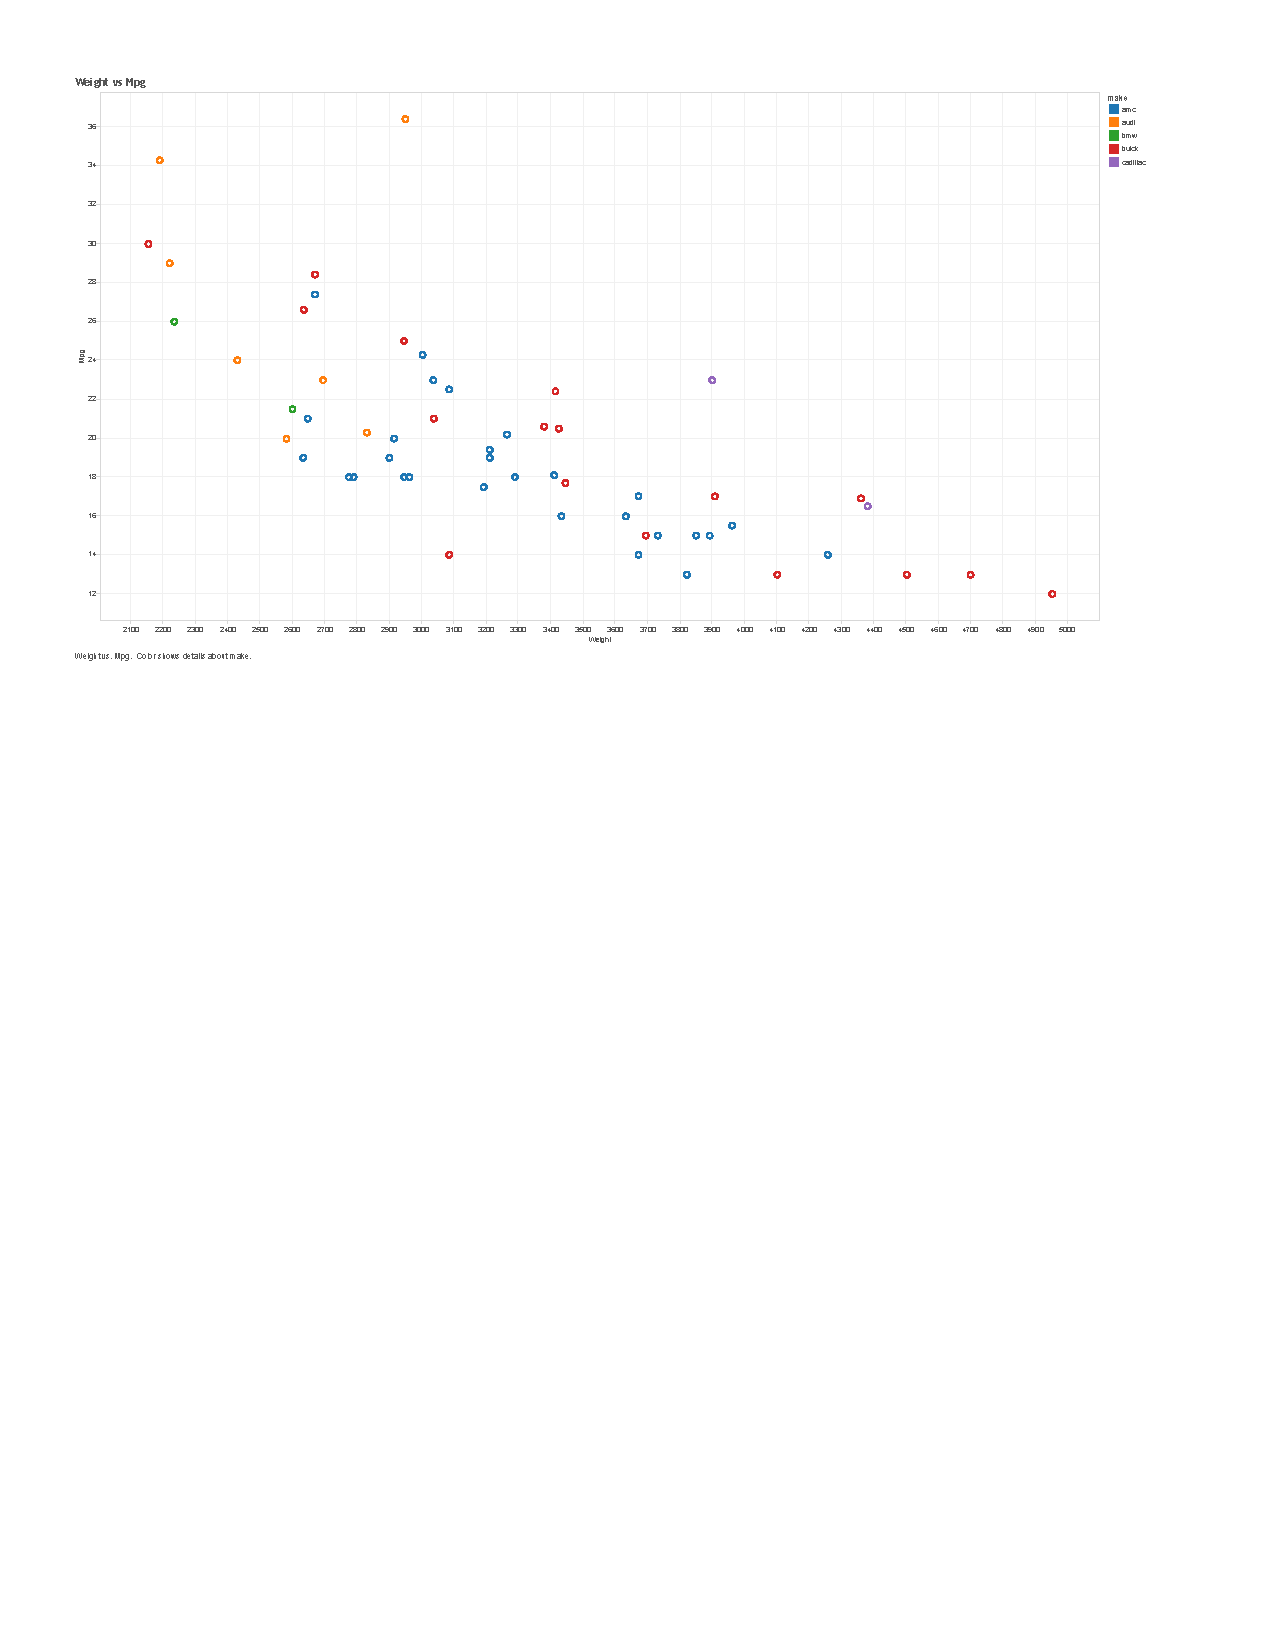
\includegraphics[max size={\textwidth}{\textheight}]{5makes}\\
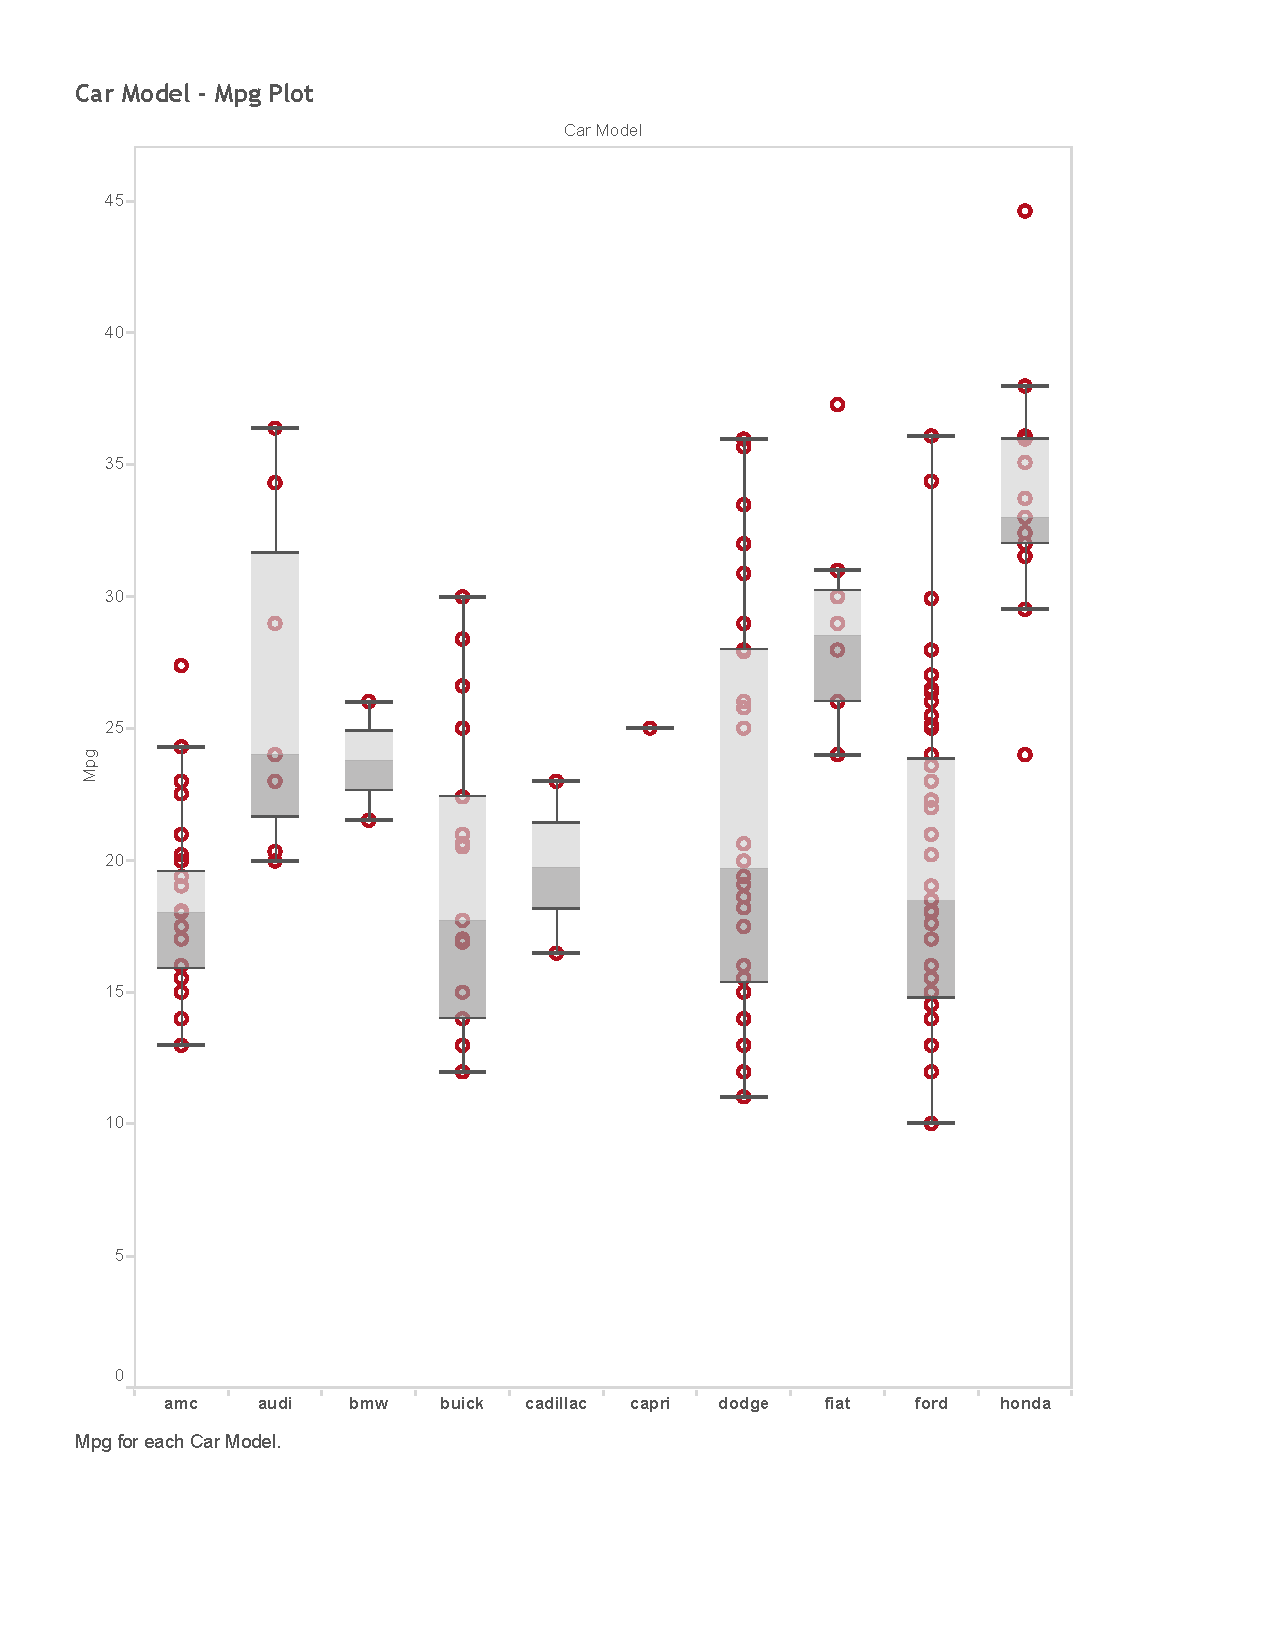
\includegraphics[max size={\textwidth}{\textheight}]{10makes}\\

}
%%% END SUBSECTION 1 %%%%%%%%%%%%%%%%%%%%%%%%%%%%%%%%%%%%%%


\subsection{Section 2}{Pick 3 data sets of your choice from UCI Machine Learning Repository. Visualize each the data set in meaningful ways that show hidden patterns. Experiment with colors, size, shapes, filters,groups and sets. Feel free to experiment with other advanced functionalities of Tableau.\\
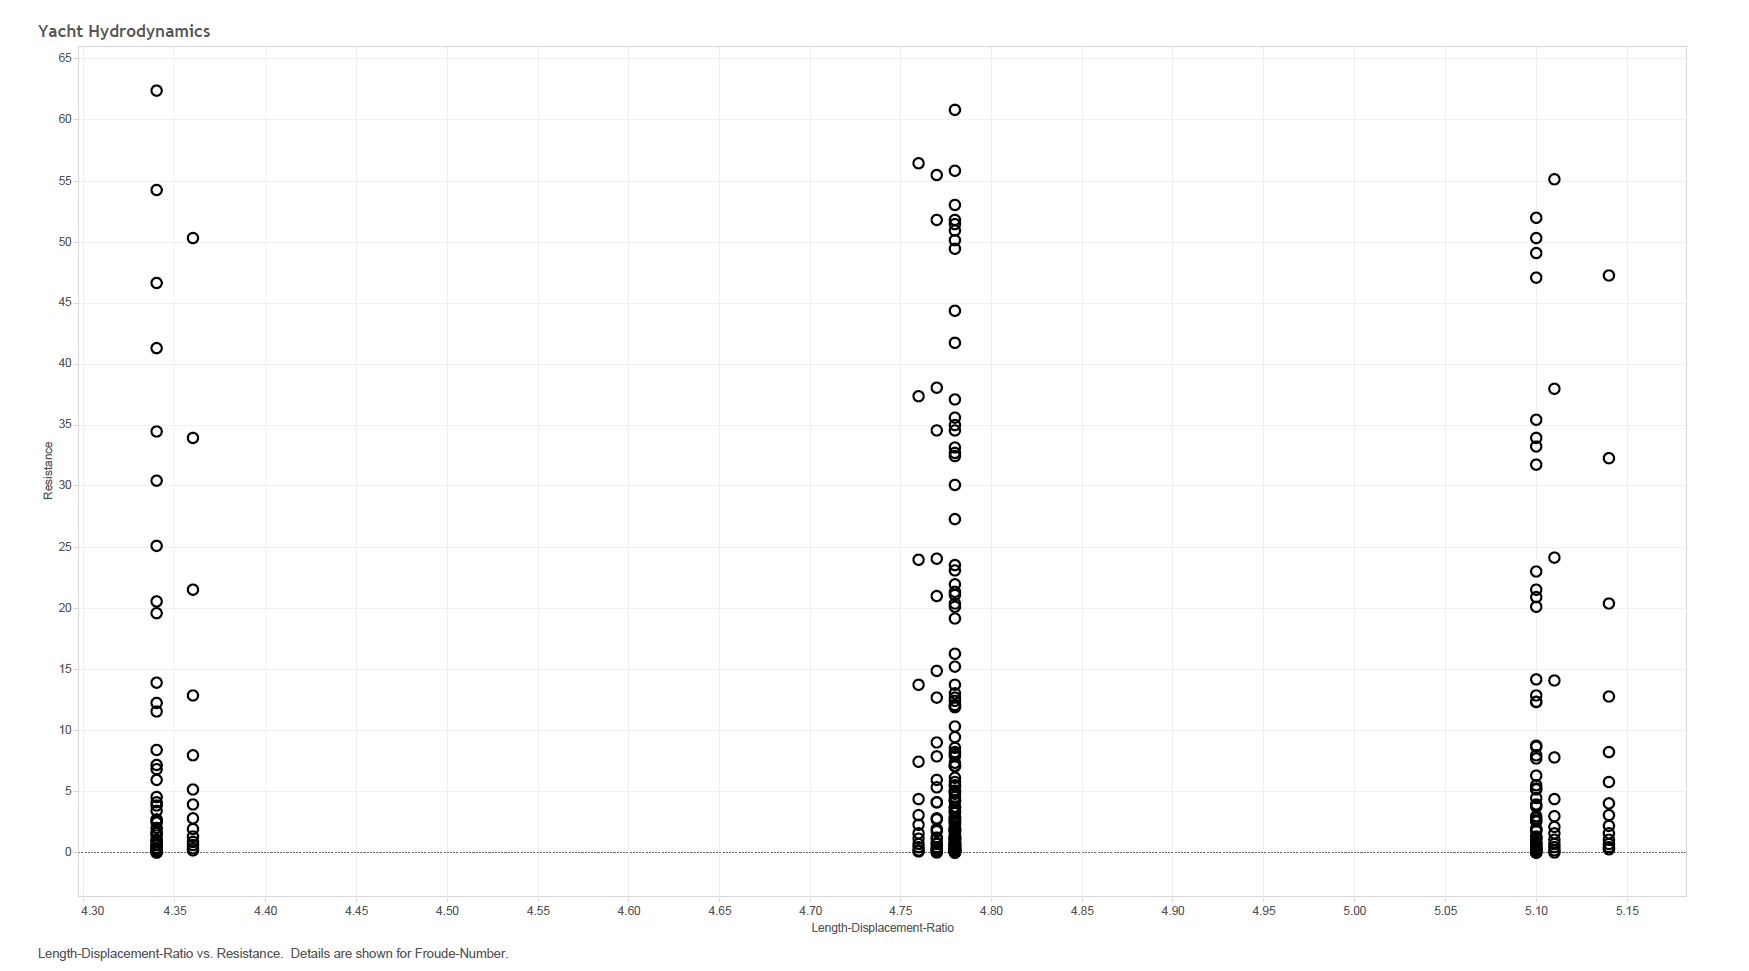
\includegraphics[max size={\textwidth}{\textheight}]{q3b-yacht}\\
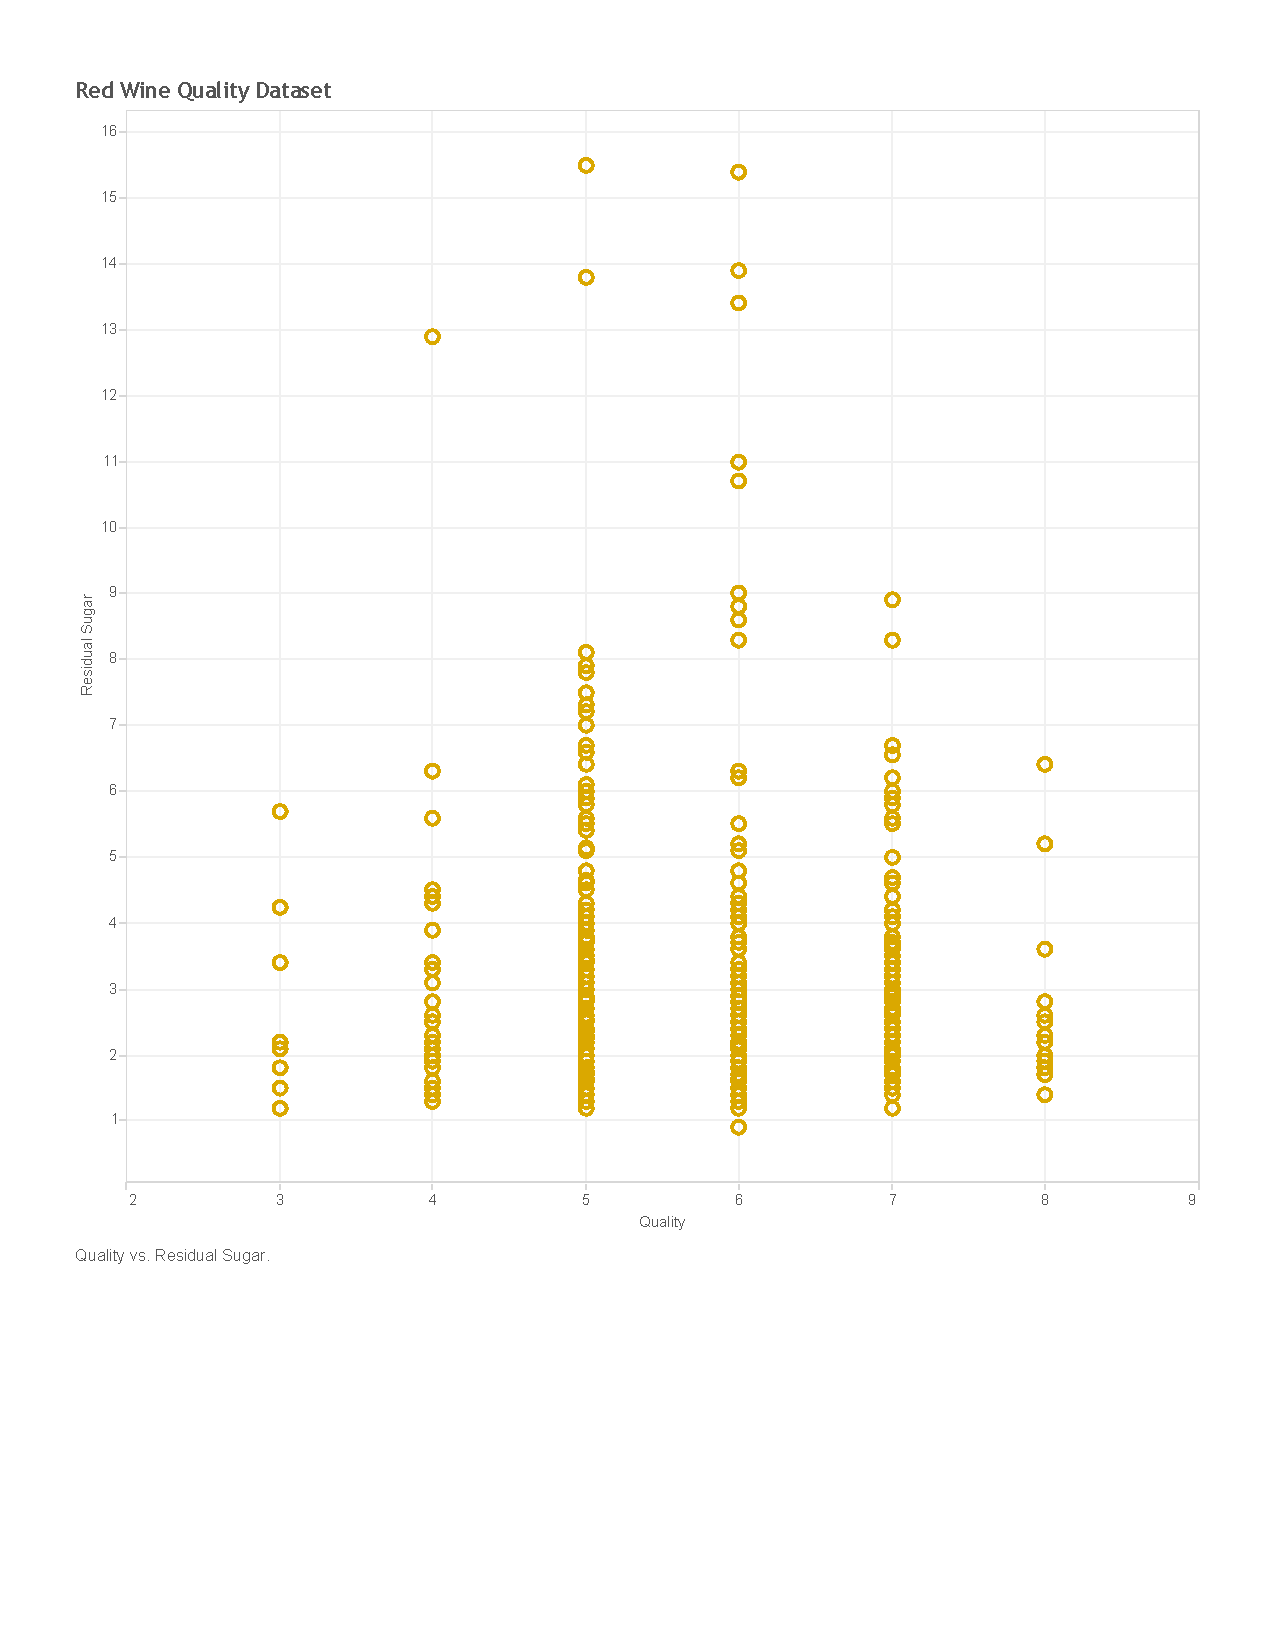
\includegraphics[max size={\textwidth}{\textheight}]{red-wine}\\
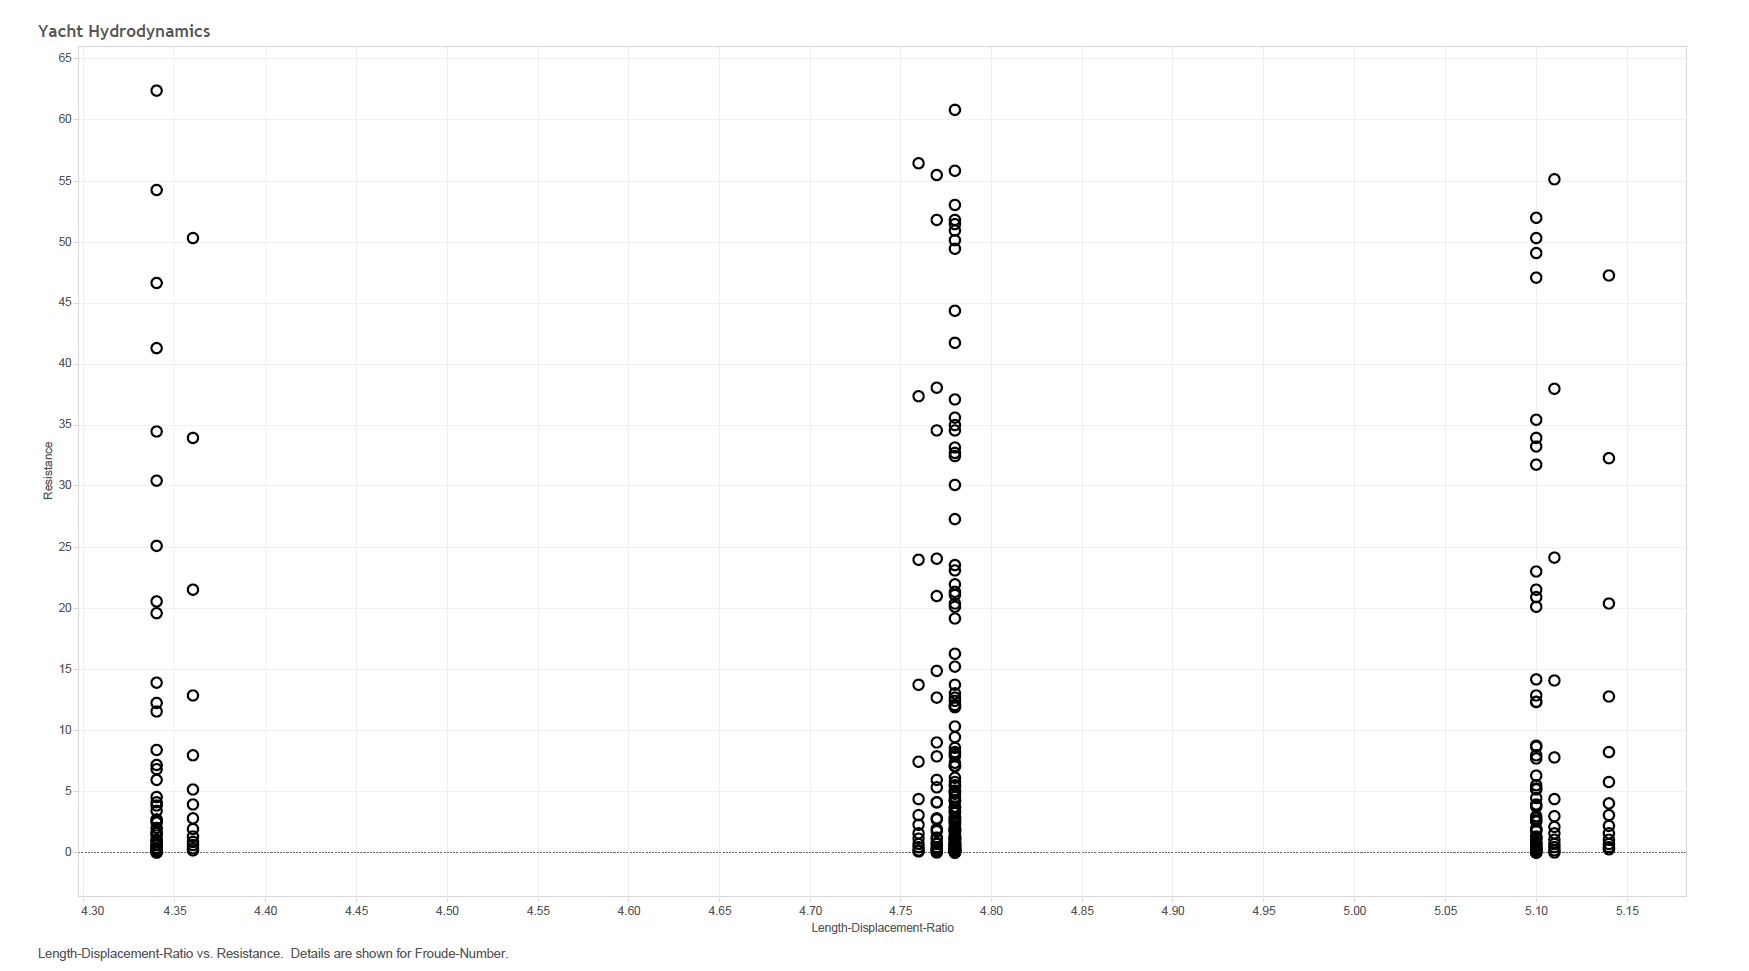
\includegraphics[max size={\textwidth}{\textheight}]{q3b-yacht}\\
}
%%% END SUBSECTION 2 %%%%%%%%%%%%%%%%%%%%%%%%%%%%%%%%%%%%%%

\subsection{Section 3}{ Tell us about your experience with Tableau. What did you learn? What did you like/dislike about Tableau?
}
%%% END SUBSECTION 4 %%%%%%%%%%%%%%%%%%%%%%%%%%%%%%%%%%%%%%
%%% END SECTION 3 %%%%%%%%%%%%%%%%%%%%%%%%%%%%%%%%%%%%%%%



\end{document}